\documentclass[11pt,a4paper]{article}

\usepackage{pifont}
\usepackage{amsmath}
\usepackage{amssymb}
\usepackage{psfig}
\usepackage{graphicx}
\usepackage{array}
\usepackage{fancyheadings}
\usepackage{here}
\usepackage{eepic,epic}
\usepackage[english]{babel}

\input{YRpersdf}

\oddsidemargin -0.4cm
\evensidemargin -0.4cm
\topmargin -1cm
\textheight 22.5cm
\textwidth 16.6cm
\headheight 1.0cm

% principal notations



\begin{document}

\begin{center}
  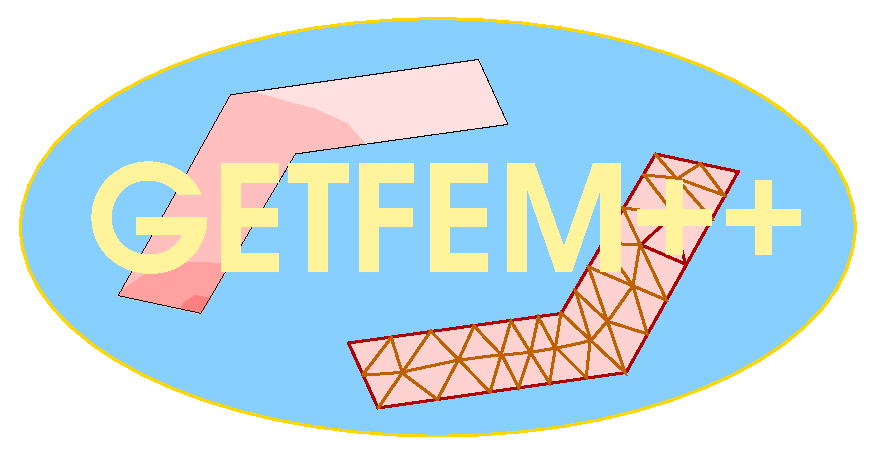
\includegraphics[width=10cm,angle=0]{getfem_logo.eps}\\[0.2cm]
  a Generic Finite Element library in C++ \\[0.5cm]
  \begin{largebox} \begin{center}
      \Huge \sc Description of Finite Element and Integration Methods
  \end{center}  \end{largebox}
  \\[0.5cm]
  { \large Yves \sc Renard\footnote{ \it MIP, INSAT, Complexe scientifique de Rangueil, 31077 Toulouse, France, Yves.Renard@gmm.insa-tlse.fr } } \\[1.0cm]
      July 31, 2002\\[1.0cm]
\end{center}

% \begin{abstract}
% Basic description of the structure of the finite element kernel of GETFEM++.
% \end{abstract}


%%%%%%%%%%%%%%%%%%%%%%%%%%%%%%%%%%%%%%%%%%%%%%%%%%%%%%%%%%%%%%%%%%%%%%%%%
%          INTRODUCTION                                                 %
%%%%%%%%%%%%%%%%%%%%%%%%%%%%%%%%%%%%%%%%%%%%%%%%%%%%%%%%%%%%%%%%%%%%%%%%%

\section*{Introduction}
This documentation describes the different finite element methods and approximative integration methods available in GETFEM++.\\[4cm]
Copyright (C) 2002\\
The program GETFEM++ is free software; you can redistribute it and/or modify
it under the terms of the GNU General Public License as published by
the Free Software Foundation; version 2 of the License.
This program is distributed in the hope that it will be useful,
but WITHOUT ANY WARRANTY; without even the implied warranty of
MERCHANTABILITY or FITNESS FOR A PARTICULAR PURPOSE.  See the
GNU General Public License for more details.
You should have received a copy of the GNU General Public License
along with this program; if not, write to the Free Software Foundation,
Inc., 59 Temple Place - Suite 330, Boston, MA  02111-1307, USA.

\newpage
\tableofcontents
\newpage

\section{Finite element methods}

all finite element methods defined in GETFEM++ are interfaced in the file {\tt getfem\_fem.h}.

\subsection{Finite element methods description}

A finite element method is defined on a reference element $\overline{T} \subset \Reel^P$ by a set of $n_d$ nodes $a^i$ and corresponding base functions 
$$ \overline{\varphi}^i : \overline{T} \subset \Reel^P \longrightarrow \Reel^Q, $$
Denoting
$$ \tilde{\varphi}^i(x) = \overline{\varphi}^i(\overline{x}) = \overline{\varphi}^i(\tau^{-1}(x)), $$
a linear transformation is allowed for the real base function
$$ \varphi^i(x) = \sum_{j = 0}^{n_d - 1} M_{ij} \tilde{\varphi}^j(x), $$
where $M$ is a $n_d \times n_d$ matrix possibly depending on the geometric transformation (i.e. on the real element).
We denote
$$ [\overline{\varphi}(\overline{x})] = \vecfour{\overline{\varphi}^0(\overline{x})}{\overline{\varphi}^1(\overline{x})}{...}{\overline{\varphi}^{n_d-1}(\overline{x})}, $$
the $n_d \times Q$ matrix, such that when a function is defined by
$$ f(x) = \sum_{i = 0}^{n_d - 1} \alpha_i \varphi^i(x), $$
one has
$$ \fbox{$\hspace{1em} f(\tau(\overline{x})) = \alpha^T M [\overline{\varphi}(\overline{x})],\hspace{1em}$} $$
where $\alpha$ is the vector of components $\alpha_i$.

\subsubsection{graphical codification of d.o.f.}

\begin{figure}[H] \label{fig:symbols}
  \begin{center}
    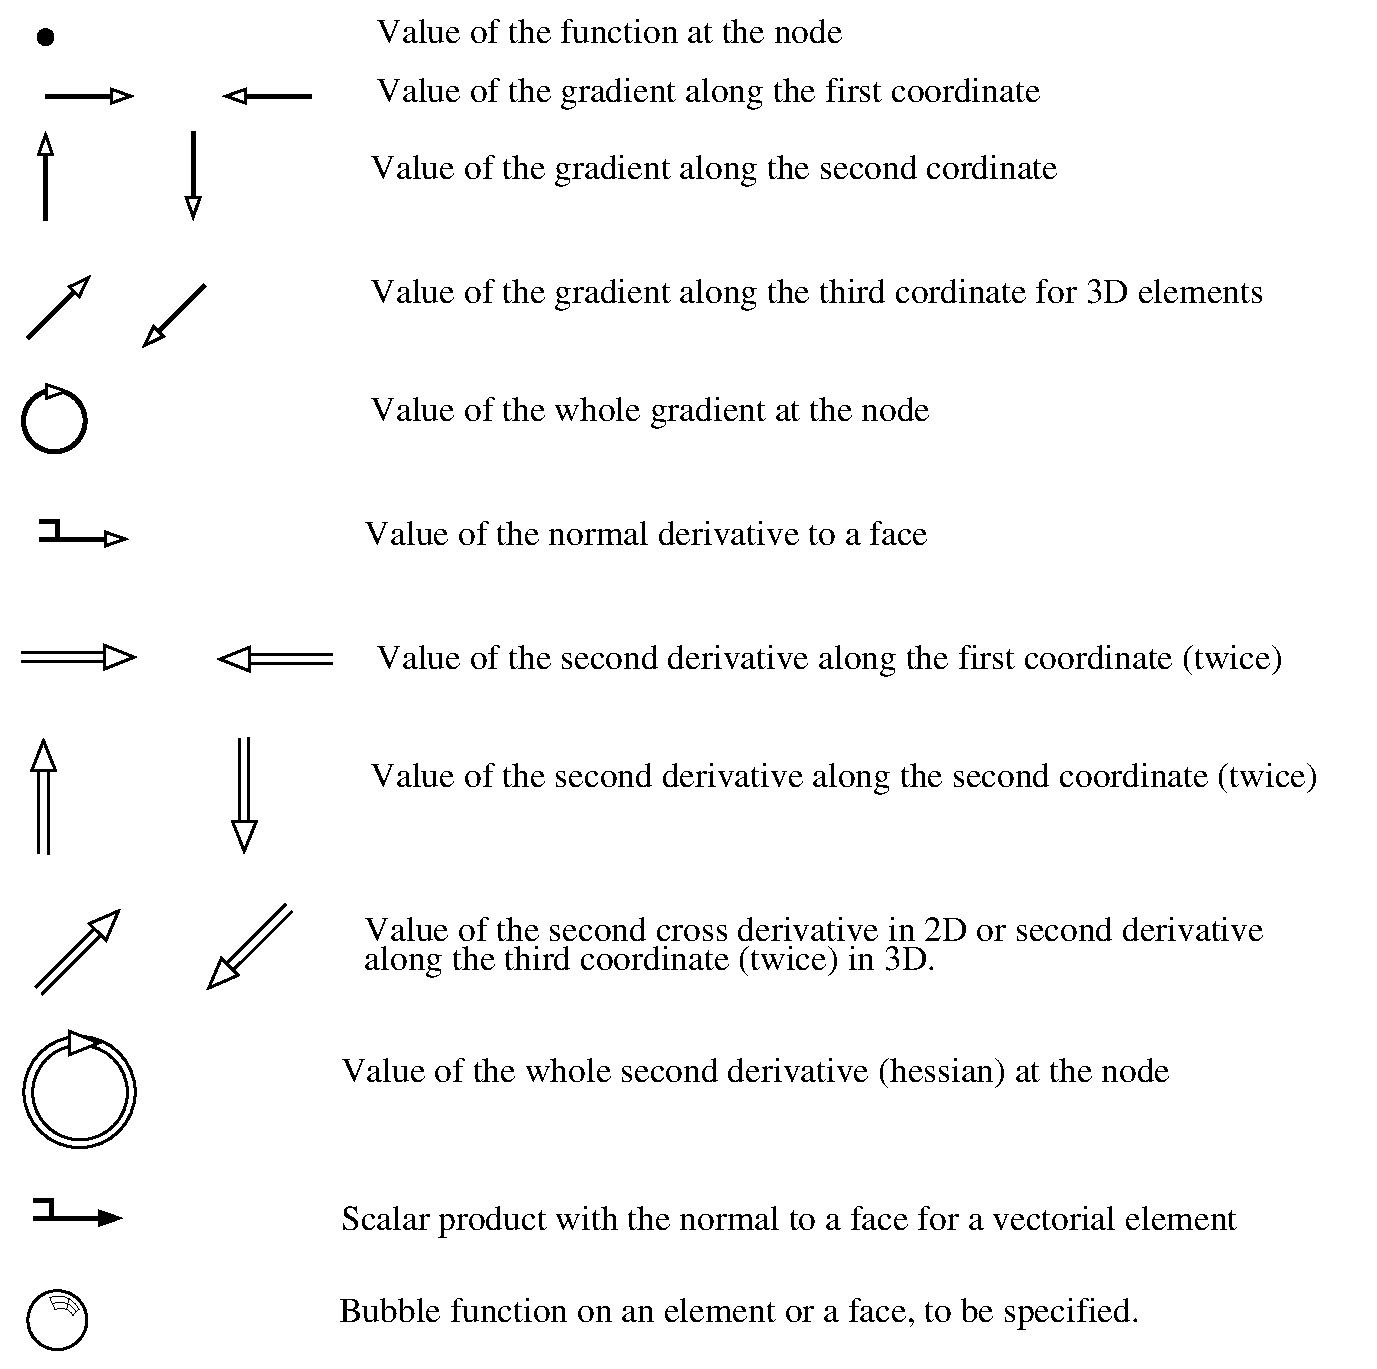
\includegraphics[width=13cm,angle=0]{getfemlist_symbols.eps}
  \end{center}
  \caption{ \it Symbols representing degree of freedom types}
\end{figure}

% a chaque �l�ment : 
% dessin des ddl avec code
% nb de ddl, degre, equivalence via la transformation g�ometrique, vectoriel ou non, analyse du raccord

\subsection{Classical ``$P_K$'' Lagrange elements on simplexes}

It is possible to define a classical ``$P_K$'' Lagrange element of arbitrary dimension and arbitrary degree. This element has only degrees of freedom which corresponds to the value of the function on a node. The grid of node is the so-called Lagrange grid. Figures \ref{fig:segmentpk}, \ref{fig:trianglepk} and \ref{fig:tetrahedronpk} show examples in dimension 1, 2 and 3.

\begin{figure}[H] 
  \begin{center} 
    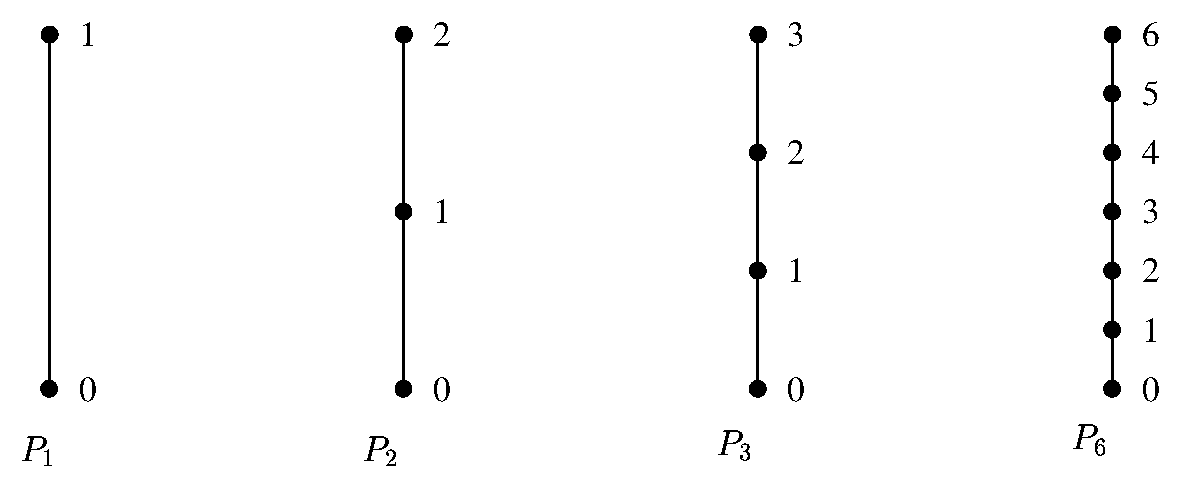
\includegraphics[width=14cm,angle=0]{getfemlist_segment_Pk.eps}
    \caption{ \it Examples of classical $P_K$ Lagrange element on a segment.} \label{fig:segmentpk}
  \end{center}
\end{figure}


\begin{figure}[H]
  \begin{center} \begin{tabular}{m{7cm}m{7cm}}
    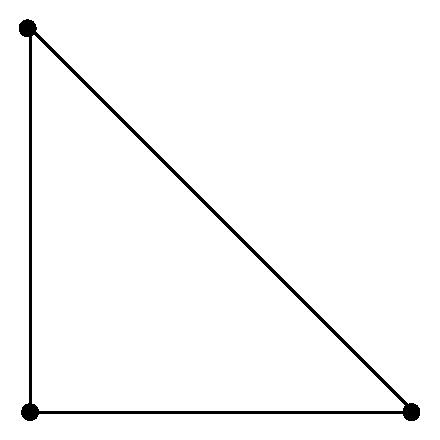
\includegraphics[width=5cm,angle=0]{getfemlist_triangle_P1.eps} & 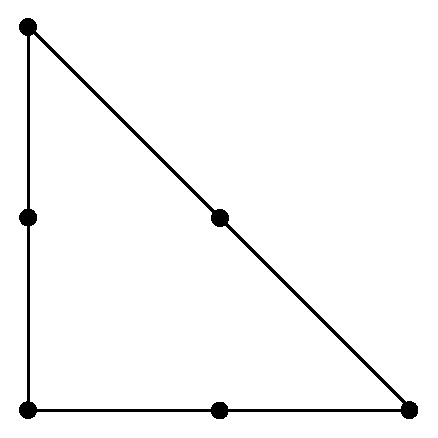
\includegraphics[width=5cm,angle=0]{getfemlist_triangle_P2.eps} \\
    $P_1$ element, 3 d.o.f., $C^0$ & $P_2$ element, 6 d.o.f., $C^0$ \\ \\
    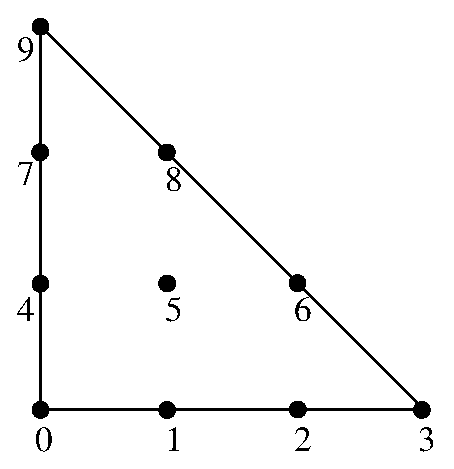
\includegraphics[width=5cm,angle=0]{getfemlist_triangle_P3.eps} & 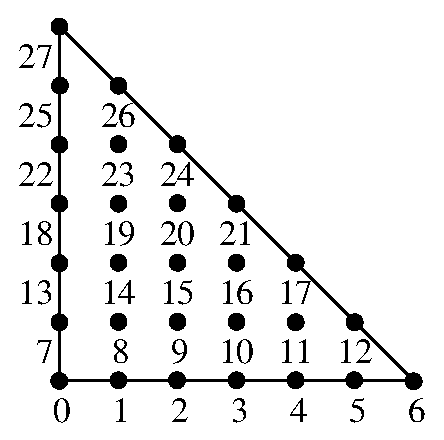
\includegraphics[width=5cm,angle=0]{getfemlist_triangle_P6.eps} \\
    $P_3$ element, 10 d.o.f., $C^0$ & $P_6$ element, 28 d.o.f., $C^0$
  \end{tabular} \end{center}
  \caption{ \it Examples of classical $P_K$ Lagrange element on a triangle.} \label{fig:trianglepk}
\end{figure}

The number of degree of freedom for a classical ``$P_K$'' Lagrange element in dimension $N$ and degree $K$ is $\Frac{(N+S)!}{N!S!}$. For instance, in dimension 2 ($N = 2$), this value is $\Frac{(N+1) (N+2)}{2}$, in dimension 3 ($N = 2$), this value is $\Frac{(N+1) (N+2) (N+3)}{6}$ ...

\begin{figure}[H]
  \begin{center}
    \begin{tabular}{m{7cm}m{7cm}}
      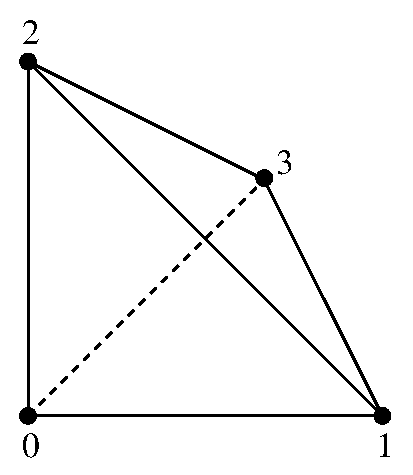
\includegraphics[width=5cm,angle=0]{getfemlist_tetrahedron_P1.eps} & 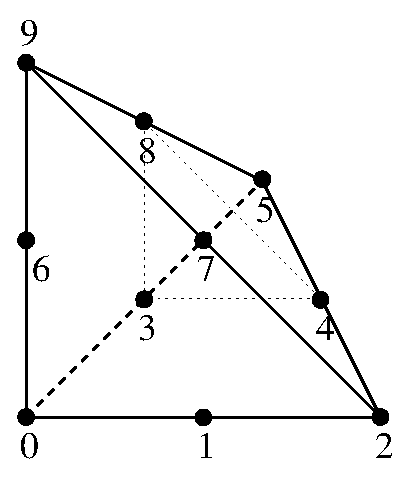
\includegraphics[width=5cm,angle=0]{getfemlist_tetrahedron_P2.eps} \\
      $P_1$ element, 4 d.o.f., $C^0$, & $P_2$ element, 10 d.o.f., $C^0$
    \end{tabular}
     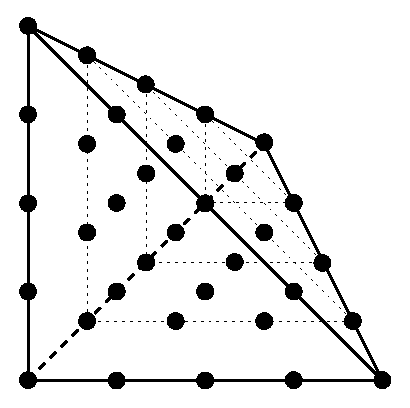
\includegraphics[width=5cm,angle=0]{getfemlist_tetrahedron_P4.eps} \\
     $P_4$ element, 35 d.o.f., $C^0$
  \end{center}
  \caption{ \it Examples of classical $P_K$ Lagrange element on a tetrahedron.} \label{fig:tetrahedronpk}
\end{figure}

The particular way selected in GETFEM++ to numerate the nodes are also shown in figures \ref{fig:segmentpk}, \ref{fig:trianglepk} and \ref{fig:tetrahedronpk}. Using another numeration, let 
$$ i_0, i_1, ... i_N, $$
be somme indexes such that
$$ 0 \le i_0, i_1, ... i_N \le K, $$
$$ \sum_{n = 0}^{N} i_n = K.$$
Then, the coordinate of a node could be defined as
$$ a_{i_0, i_1, ... i_N} = \sum_{n = 0}^{N} \Frac{i_n}{K}P_n, $$
where $P_0, P_1, ... P_N$ are the vertexes of the simplex.
Then each base function, corresponding of each node $a_{i_0, i_1, ... i_N}$ is defined as
$$ \phi_{i_0, i_1, ... i_N} = \prod_{n = 0}^{N} \prod_{j=0}^{i_n-1} \left(\Frac{K \lambda_n - j}{j+1}\right).$$
where $\lambda_n$ is the barycentric coordinate, i.e. the polynomial of order 1 whose value is $1$ on the vertex $P_n$ and whose value is $0$ on the other vetices. On the reference element, one has
$$ \lambda_n = x_n, \ \ 0 \le n < N, $$
$$ \lambda_N = 1 - x_0 - x_1 - ... - x_{N-1}. $$

When between two elements of the same order (even with different dimensions), the degrees of freedom of a common face are linked, the element is of class $C^0$. This mean that the global polynomial is continuous. If you try to link elements of different orders, you will get some trouble with the unlinked degrees of freedom. This is not automatically supported by GETFEM++, so you will have to support it (add constraints on this degrees of freedom).\\[0.5cm] 

For some applications (computation of a gradient for instance) one does not want the degrees of freedom of a common face to be linked. This is why there are two versions of the classical ``$P_K$'' Lagrange element. The function\\[0.5cm]
{\tt getfem::ppolyfem getfem::PK\_fem(N, K)}\\[0.5cm]
return the description of the linkable element, and\\[0.5cm]
 {\tt getfem::ppolyfem getfem::PK\_discontinuous\_fem(N, K)}\\[0.5cm]
return the description of the unlinkable element.

\subsection{Classical Lagrange elements on other geometries}

to be done ...

\subsection{Specific elements in dimension 1}

to be done ...

\subsection{Specific elements in dimension 2}

\begin{figure}[H]
  \begin{center}
    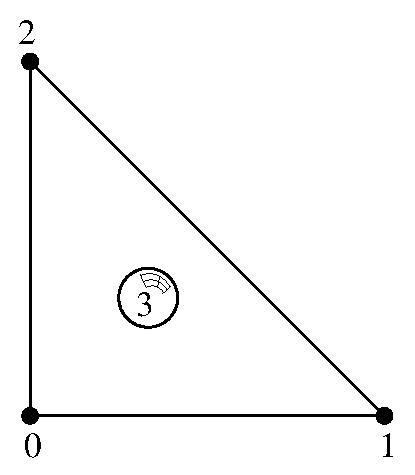
\includegraphics[width=5cm,angle=0]{getfemlist_triangle_P1_bubble.eps}
  \end{center}
  \caption{ \it$P_1$ Lagrange element on a triangle with additional bubble function, 4 d.o.f., $C^0$} 
  \label{fig:triangle_p1_bubble}
\end{figure}

to be described ...

\begin{figure}[H]
  \begin{center}
    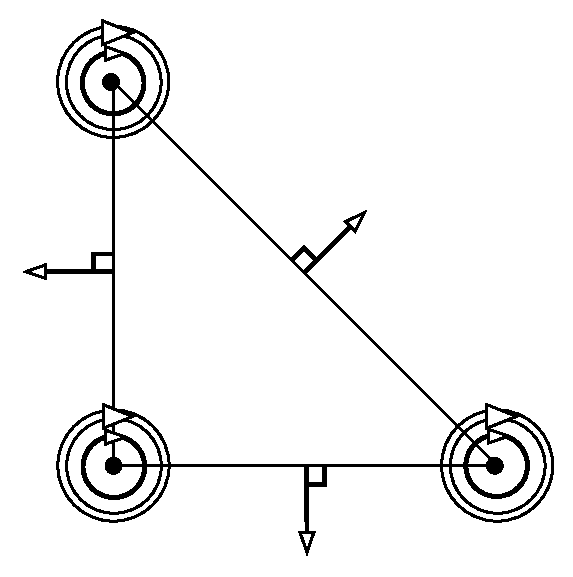
\includegraphics[width=6cm,angle=0]{getfemlist_argyris.eps}
  \end{center}
  \caption{ \it Argyris element, $P_5$, 21 d.o.f., $C^1$}
  \label{fig:argyris}
\end{figure}
to be done ...

\subsection{Specific elements in dimension 3}

to be done ...

\subsection{Tensorial product of elements}

to be done ...

\subsection{What really means arbitrary geometric transformation}

(graphics ...)

\section{Integration methods}

\subsection{Integration methods description}

The integrations methods are of two kinds. The file {\tt bgeot\_poly\_integration.h} defines exact integrations of polynomials and the file {\tt bgeot\_approx\_integration.h} defines approximated integrations of any function. The exact integration can only be used if all the elements are polynomial and if the geometric transformation is linear.

In the file {\tt bgeot\_poly\_integration.h} the following functions are defined

\begin{center} \begin{tabular}{|m{0.55\linewidth}|m{0.4\linewidth}|} \hline
{\tt "IM\_EXACT\_SIMPLEX(n)"} & Description of the exact integration of polynomials on the simplex of reference of dimension {\tt n}. \\ \hline
\end{tabular}  
\begin{tabular}{|m{0.55\linewidth}|m{0.4\linewidth}|} \hline
{\tt "IM\_PRODUCT(a, b)"} & Description of the exact integration on the convex which is the direct product of the convex in {\tt a} and in {\tt b}.\\ \hline
\end{tabular}  
\begin{tabular}{|m{0.55\linewidth}|m{0.4\linewidth}|} \hline
{\tt "IM\_EXACT\_PARALLELEPIPED(n)"} & Description of the exact integration of polynomials on the parallelepiped of reference of dimension {\tt n}\\ \hline
\end{tabular}  
\begin{tabular}{|m{0.55\linewidth}|m{0.4\linewidth}|} \hline
{\tt "IM\_EXACT\_PRISM(n)"} & Description of the exact integration of polynomials on the prism of reference of dimension {\tt n}\\ \hline
\end{tabular} \end{center}


Even though a description of exact integration method exists on parallelepipeds or prisms, most of the time the geometric transformations on such elements are not linear and the exact integration cannot be used.

In the file {\tt bgeot\_approx\_integration.h} the following functions are defined

\begin{center} \begin{tabular}{|m{0.55\linewidth}|m{0.4\linewidth}|} \hline
{\tt "IM\_GAUSS1D(k)" } & Description of the Gauss integration on a segment of order {\tt k}. \\ \hline
\end{tabular}  
\begin{tabular}{|m{0.55\linewidth}|m{0.4\linewidth}|} \hline
{\tt "IM\_NC(n,k)"} & Description of the integration on a simplex of reference of dimension {\tt n} for polynomials of degree {\tt k} with the Newton Cotes method (based on Lagrange interpolation).\\ \hline
\end{tabular}  
\begin{tabular}{|m{0.55\linewidth}|m{0.4\linewidth}|} \hline
{\tt "IM\_PRODUCT(a,b)"} & Build a method doing the direct product of methods {\tt a} and {\tt b}. \\ \hline
\end{tabular}  
\begin{tabular}{|m{0.55\linewidth}|m{0.4\linewidth}|} \hline
{\tt "IM\_TRIANGLE(2)"} & Integration on a triangle of order 2 with 3 points. \\ \hline
\end{tabular}
\begin{tabular}{|m{0.55\linewidth}|m{0.4\linewidth}|} \hline
{\tt "IM\_TRIANGLE(7)"} & Integration on a triangle of order 7 with 13 points. \\ \hline
\end{tabular} 
\begin{tabular}{|m{0.55\linewidth}|m{0.4\linewidth}|} \hline
{\tt "IM\_QUAD(2)"} & Integration on quadrilaterals of order 2 with 3 points. \\ \hline
\end{tabular}
\begin{tabular}{|m{0.55\linewidth}|m{0.4\linewidth}|} \hline
{\tt "IM\_TETRAHEDRON(5)"} & Integration on a tetrahedron of order 5 with 15 points. \\ \hline
\end{tabular} \end{center}


Other methods can be easily defined.

\subsection{Exact Integration methods}

to be done ...

\subsection{Newton cotes Integration methods}
to be done ...


\subsection{Gauss Integration methods on dimension 1}

to be done ...

\subsection{Gauss Integration methods on dimension 2}

to be done ...

\subsection{Gauss Integration methods on dimension 3}

to be done ...

\subsection{Direct product of integration methods}


to be done ...

\begin{thebibliography}{99}
% \bibliographystyle{apalike}
% \bibliographystyle{plain}
% \bibliography{all}
\bibitem{dh-to1984} 
  G. {\sc Dhatt, and  G. Touzot}
  {\it The Finite Element Method Displayed}, 
 J. Wiley \& Sons,  New York, 1984.

\bibitem{BAS_COMP}
  Y. {\sc Renard},
  {\it Elementary Computations in GETFEM++}, 2002.

\bibitem{USER_DOC}
  Y. {\sc Renard},
  {\it Short User Documentation of GETFEM++}, 2002.

\bibitem{nedelec1991}
  J.-C. {\sc Nedelec},
  {\it Notions sur les techniques d'�l�ments finis}, Ellipses, SMAI, Math�matiques \& Applications n�7, 1991.
\end{thebibliography}


\end{document}
